\chapter{Calibration du modèle} 

\lettrine{I}{l} est question ici de définir la méthodologie afin de calibrer les paramètres libres du modèle.
On s'intéressera notamment à définir une fonction de coût, pour évaluer la qualité de la calibration.
Dans cette optique, on essayera de calibrer les paramètres en utilisant uniquement les dynamiques du verger n\textdegree1 ; le deuxième servira à la validation.

Il peut être utile de donner la liste des paramètres à calibrer :
\begin{itemize}
 \item $\gamma$, le paramètre relatif à l'arrivée des femelles exogènes ;
 \item $p_{\text{m}}$, le paramètre relatif à la migration des femelles endogènes entre les sous-parcelles ;
 \item $\mu^{1}_{\text{ER}}$ et $\mu^{2}_{\text{ER}}$, les probabilité de réussir à entrer et à sortir du sol pour les cécidomyies pour la modalité «enherbement ras». Pour simplifier,
 on pose $\mu^{1}_{\text{ER}} = \mu^{2}_{\text{ER}}$;
 \item $\mu^{1}_{\text{EH}}$ et $\mu^{2}_{\text{EH}}$, les probabilité de réussir à entrer et à sortir du sol pour les cécidomyies pour la modalité «enherbement haut». Ici aussi,
 on pose $\mu^{1}_{\text{EH}} = \mu^{2}_{\text{EH}}$;
 \item $k$, le paramètre relatif à la disponibilité en ressources pour les inflorescences ;
 \item \texttt{stock}, le nombre de larves entrées en diapause les années précédentes qui décident de sortir l'année considérée ;
 \item $E_0\mu_{\ell}$, le nombre d'œufs pondus par une femelle qui survivent, se transforment en larves puis s'éjectent de l'inflorescences. 
\end{itemize}


\section{Fonction de coût}

Avant une quelconque estimation des paramètres, nous avons besoin de mesurer la qualité de nos estimations.
Pour ce faire, on utilisera une fonction pour comparer le nombre de larves estimées avec le nombre de larves observées. 
Pour définir cette fonction, on pose :
\begin{itemize}
 \item $m$, le nombre de jours entre la première observation et la dernière ;
 \item $n$, le nombre de relevés effectif;
 \item $t$, le nombre de jours passés depuis la première observation ;
 \item $t^j$, le nombre de jours entre la première observation et le $j^{\text{ème}}$ relevé.
\end{itemize}
(On a donc $t^1 = 0$ et $t^n = m$.)

La fonction est alors définie par
$$
f(y, \hat y) = \frac{\sqrt{\frac{1}{n-1}\sum_{j=2}^n\left( y^*_j - \hat y^*_j \right)^2}}{\max(y^*) - \min(y^*)},
$$
où 
$$y^*_j =  y_{t^j} \qquad \text{ et } \qquad \hat y^*_j = \frac{1}{t^j - t^{j-1}}\sum_{k=t^{j-1}}^{t^j} \hat y_k.$$
La figure~\ref{fig:calib} illustre le fonctionnement de la fonction.
Appliquer la fonction à $n-1$ valeurs (correspondant aux relevés sur le terrain) plutôt qu'à chacun des $m$ jours (correspondant à l'étendue des relevés) est motivé par le fait que les relevés ne furent pas fait à des intervalles de temps régulier.
Ce faisant, on évite d'attribuer plus d'importance aux relevés qui ont eu un écart relativement important avec le relevé précédent.

\begin{figure}[ht]
\centering
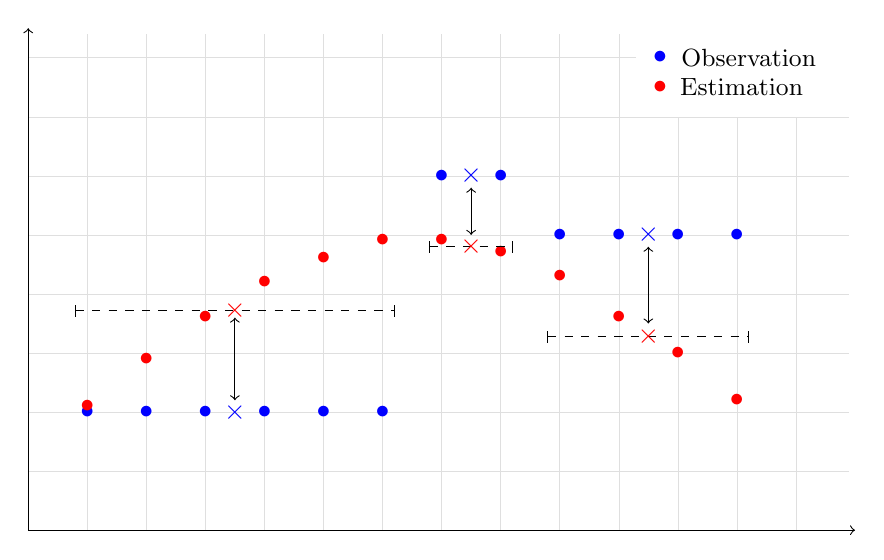
\begin{tikzpicture}[scale = 0.75]
 \draw [very thin, lightgray, opacity = 0.5] (0,0) grid (13.9, 8.4);
 \draw [->] (0, 0) -- (0, 8.5);
 \draw [->] (0, 0) -- (14, 0);
 \draw (1, 2) node{\textcolor{blue}{$\bullet$}};
 \draw (2, 2) node{\textcolor{blue}{$\bullet$}};
 \draw (3, 2) node{\textcolor{blue}{$\bullet$}};
 \draw (4, 2) node{\textcolor{blue}{$\bullet$}};
 \draw (5, 2) node{\textcolor{blue}{$\bullet$}};
 \draw (6, 2) node{\textcolor{blue}{$\bullet$}};
 \draw (7, 6) node{\textcolor{blue}{$\bullet$}};
 \draw (8, 6) node{\textcolor{blue}{$\bullet$}};
 \draw (9 , 5) node{\textcolor{blue}{$\bullet$}};
 \draw (10, 5) node{\textcolor{blue}{$\bullet$}};
 \draw (11, 5) node{\textcolor{blue}{$\bullet$}};
 \draw (12, 5) node{\textcolor{blue}{$\bullet$}};
 \draw (1, 2.1) node{\textcolor{red}{$\bullet$}};
 \draw (2, 2.9) node{\textcolor{red}{$\bullet$}};
 \draw (3, 3.6) node{\textcolor{red}{$\bullet$}};
 \draw (4, 4.2) node{\textcolor{red}{$\bullet$}};
 \draw (5, 4.6) node{\textcolor{red}{$\bullet$}};
 \draw (6, 4.9) node{\textcolor{red}{$\bullet$}};
 \draw (7, 4.9) node{\textcolor{red}{$\bullet$}};
 \draw (8, 4.7) node{\textcolor{red}{$\bullet$}};
 \draw (9, 4.3) node{\textcolor{red}{$\bullet$}};
 \draw (10, 3.6) node{\textcolor{red}{$\bullet$}};
 \draw (11, 3) node{\textcolor{red}{$\bullet$}};
 \draw (12, 2.2) node{\textcolor{red}{$\bullet$}};
 \draw [dashed] (0.8, 3.716) -- (6.2, 3.716) ;
 \draw [dashed] (6.8, 4.8) -- (8.2, 4.8) ;
 \draw [dashed] (8.8, 3.275) -- (12.2, 3.275) ;
 \draw (0.8, 3.616) -- (0.8, 3.816);
 \draw (6.2, 3.616) -- (6.2, 3.816);
 \draw (6.8, 4.7) -- (6.8, 4.9);
 \draw (8.2, 4.7) -- (8.2, 4.9);
 \draw (8.8, 3.175) -- (8.8, 3.375);
 \draw (12.2, 3.175) -- (12.2, 3.375);
 \draw (3.5, 3.716) node{\textcolor{red}{$\times$}};
 \draw (7.5, 4.8) node{\textcolor{red}{$\times$}}; 
 \draw (10.5, 3.275) node{\textcolor{red}{$\times$}};
 \draw (3.5, 2) node{\textcolor{blue}{$\times$}};
 \draw (7.5, 6) node{\textcolor{blue}{$\times$}}; 
 \draw (10.5, 5) node{\textcolor{blue}{$\times$}}; 
 \draw [<->] (3.5, 2.2) -- (3.5, 3.6);                  
 \draw [<->] (7.5, 5.8) -- (7.5, 5);
 \draw [<->] (10.5, 4.8) -- (10.5, 3.5);
 \draw [fill=white,white] (10.3, 7.01) rectangle (13.9, 8.4);
 \draw (12.2, 8) node {{\small Observation}};
 \draw (12.08, 7.5) node {{\small Estimation}};
 \draw (10.7, 8) node{\textcolor{blue}{$\bullet$}};
 \draw (10.7, 7.5) node{\textcolor{red}{$\bullet$}};
 \draw (6, 0.135) node[rotate = 180] {\textcolor{ForestGreen}{$\intercal$}};
 \draw (8, 0.135) node[rotate = 180] {\textcolor{ForestGreen}{$\intercal$}};
 \draw (12, 0.135) node[rotate = 180] {\textcolor{ForestGreen}{$\intercal$}};
\end{tikzpicture}
\caption{Schéma illustrant le fonctionnement de la fonction objectif. À chaque relevé effectif (marqueurs verts), on fait correspondre la période correspondant à ce relevé (segments en pointillés).
Et pour chacune de ces périodes, on calcule la moyenne des valeurs estimées (les croix rouges). On compare ensuite les moyennes ainsi calculées avec les valeurs observées associées (les croix bleues).}
\label{fig:calib}
\end{figure}


Par la suite, l'objectif sera de minimiser cette fonction pour chacune des sous-parcelle.

\section{Analyse de sensibilité}

Avant de calibrer le modèle, il est pertinent d'effectuer une analyse de sensibilité.
L'analyse de sensibilité est définie par \citet{saltelli} comme
\begin{quote}
 «l'étude de comment l'incertitude de la sortie d'un modèle --- qu'elle soit numérique ou non --- peut être répartie entre les différentes sources d'incertitudes que sont les entrées du modèle.»\footnote{«The study of
how uncertainty in the output of a model (numerical or otherwise) can be
apportioned to different sources of uncertainty in the model input.»}
\end{quote}
Autrement dit, on cherche à connaître les paramètres les plus influants sur la sortie du modèle.
La calibration comportant toujours une part d'arbitraire, cette analyse permet de prendre du recul sur les choix de paramètres, relativement à leur impact sur le modèle.


\section{Algorithme d'optimisation}

\section{Exploration de l'ensemble des solutions}
